\documentclass[14pt, aspectratio=169]{beamer}
\usepackage[T1]{fontenc}
\usepackage[english]{babel} % german as language
\usepackage{csquotes}
\usepackage{parskip} % for paragraph line skip

% for tables/figures
\usepackage{graphicx}
\usepackage{caption}
\usepackage{array}
\graphicspath{ {figures/} } % set path to figures
\renewcommand{\listfigurename}{Abbildungsverzeichnis}
\renewcommand{\listtablename}{Tabellenverzeichnis}

% Appendix
\usepackage[toc,page]{appendix}
\renewcommand\appendixname{Anhang} % Change name to German
\renewcommand\appendixpagename{Anhang}
\renewcommand\appendixtocname{Anhang}


% \usepackage{sectsty} -> falls section font size 14 haben muss
% \sectionfont{\large\bfseries}

% um videos einzubinden
\usepackage{hyperref}

% Citation: BibLaTeX als author-year style, benötigt xelatex->biber->xelatex(2x) als recipe!
\usepackage[
  backend=biber,
  style=authoryear
]{biblatex}
\addbibresource{refs.bib}


% Titel/Startseite
\title{KI in der Lehre}
\subtitle{Level 1: Ein Seminar für Lehrkräfte}
\author{Lukas Schaffrath}
\date{Januar 2026}

%theme
%%general
\usetheme[right]{PaloAlto}
\setbeamersize{text margin left=1em, text margin right=1em}

%%catpuccin
\definecolor{ctpRosewater}{HTML}{F5E0DC}
\definecolor{ctpFlamingo}{HTML}{F2CDCD}
\definecolor{ctpPink}{HTML}{F5C2E7}
\definecolor{ctpMauve}{HTML}{CBA6F7}
\definecolor{ctpRed}{HTML}{F38BA8}
\definecolor{ctpMaroon}{HTML}{EBA0AC}
\definecolor{ctpPeach}{HTML}{FAB387}
\definecolor{ctpYellow}{HTML}{F9E2AF}
\definecolor{ctpGreen}{HTML}{A6E3A1}
\definecolor{ctpTeal}{HTML}{94E2D5}
\definecolor{ctpSky}{HTML}{89DCEB}
\definecolor{ctpSapphire}{HTML}{74C7EC}
\definecolor{ctpBlue}{HTML}{89B4FA}
\definecolor{ctpLavender}{HTML}{B4BEFE}
\definecolor{ctpText}{HTML}{CDD6F4}
\definecolor{ctpSubtext1}{HTML}{BAC2DE}
\definecolor{ctpSubtext0}{HTML}{A6ADC8}
\definecolor{ctpOverlay2}{HTML}{9399B2}
\definecolor{ctpOverlay1}{HTML}{7F849C}
\definecolor{ctpOverlay0}{HTML}{6C7086}
\definecolor{ctpSurface2}{HTML}{585B70}
\definecolor{ctpSurface1}{HTML}{45475A}
\definecolor{ctpSurface0}{HTML}{313244}
\definecolor{ctpBase}{HTML}{1E1E2E}
\definecolor{ctpMantle}{HTML}{181825}
\definecolor{ctpCrust}{HTML}{11111B}

% Main colors
\setbeamercolor{background canvas}{bg=ctpBase}
\setbeamercolor{normal text}{fg=ctpText,bg=ctpBase}
\setbeamercolor{frametitle}{fg=ctpMauve,bg=ctpBase}
\setbeamercolor{title}{fg=ctpBlue,bg=ctpBase}
\setbeamercolor{author}{fg=ctpText}
\setbeamercolor{date}{fg=ctpSubtext1}
\setbeamercolor{section in toc}{fg=ctpMauve}
\setbeamercolor{structure}{fg=ctpMauve}

% Items
\setbeamercolor{itemize item}{fg=ctpLavender}
\setbeamercolor{itemize subitem}{fg=ctpSapphire}
\setbeamercolor{enumerate item}{fg=ctpLavender}

% Blocks
\setbeamercolor{block title}{fg=ctpYellow,bg=ctpSurface1}
\setbeamercolor{block body}{fg=ctpText,bg=ctpSurface0}

% Buttons and links
\setbeamercolor{button}{bg=ctpBlue,fg=ctpBase}
\hypersetup{
    colorlinks=true,
    linkcolor=ctpSky,
    urlcolor=ctpTeal
}

% Sidebar colors
\setbeamercolor{sidebar}{bg=ctpSurface0}
\setbeamercolor{sidebar right}{bg=ctpSurface0}
\setbeamercolor{title in sidebar}{fg=ctpSky}
\setbeamercolor{author in sidebar}{fg=ctpSubtext1}
\setbeamercolor{section in sidebar}{fg=ctpText,bg=ctpSurface1}
\setbeamercolor{section in sidebar shaded}{fg=ctpSubtext1,bg=ctpSurface0}
\setbeamercolor{subsection in sidebar}{fg=ctpSapphire}
\setbeamercolor{subsection in sidebar shaded}{fg=ctpOverlay1}

% Palette colors
\setbeamercolor{palette sidebar primary}{fg=ctpSky,bg=ctpSurface0}
\setbeamercolor{palette sidebar secondary}{fg=ctpMauve,bg=ctpSurface0}
\setbeamercolor{palette sidebar tertiary}{fg=ctpText,bg=ctpSurface0}
\setbeamercolor{palette sidebar quaternary}{fg=ctpSubtext1,bg=ctpSurface0}

% Headline (die Box oben) - dunkler Hintergrund
\setbeamercolor{section in head/foot}{fg=ctpMauve,bg=ctpSurface1}
\setbeamercolor{subsection in head/foot}{fg=ctpText,bg=ctpSurface1}

% Templates
\setbeamertemplate{navigation symbols}{}
\setbeamertemplate{frametitle continuation}{}
\setbeamertemplate{section in sidebar shaded}[default]

% Frame-Titel ein wenig kleiner machen
\setbeamerfont{frametitle}{size=\large}

\makeatletter
\setbeamertemplate{headline}{%
  \ifnum\theframenumber=1\relax
    % Auf Titelseite: keine Headline
  \else
    % Auf anderen Seiten: Sektion anzeigen
    \begin{beamercolorbox}[wd=\paperwidth,ht=4ex,dp=2ex,leftskip=1em]{section in head/foot}
      \usebeamerfont{section in head/foot}\insertsectionhead
    \end{beamercolorbox}
  \fi
}
\makeatother

% make each text appear after another!!
% \beamerdefaultoverlayspecification{<+->}

% Start des Dokuments
\begin{document}

% =====================================================
% TITEL
% =====================================================

\maketitle

% =====================================================
% SECTION 0 – EINLEITUNG
% =====================================================

\section{Einleitung}

\begin{frame}{}
  \begin{center}
    \Huge Kurz zu mir\\
    \vspace{0.4cm}
    \Large Wer spricht hier eigentlich?
  \end{center}
\end{frame}

\begin{frame}{Mein Hintergrund}
\begin{itemize}
    \item Webentwickler und IT-Administrator
    \item Lehramtsstudent (B.\,A./M.\,Ed.) (RWTH Aachen)
    \item Studium: Cognitive, Digital and Empirical English Studies (RWTH Aachen)
    \item Aktuelle Forschung: KI in der Lehre
\end{itemize}
\end{frame}

\begin{frame}{Warum ich?}
\begin{itemize}
    \item Mehrjährige Unterrichtserfahrung (u.\,a. Kleingruppen)
    \item Entwicklung digitaler Lernplattformen und Kurse
    \item Arbeit mit Studierenden und Lehrenden
\end{itemize}
\textbf{-> Brücke zwischen Technik und Lehre}
\end{frame}

\begin{frame}{Warum ich?}
\begin{itemize}
    \item Eigene empirische Forschung zu KI-generierten Texten
    \item Beratung zu KI-Einsatz und Datenschutz
    \item Kontinuierliche Auseinandersetzung mit aktueller Forschung
\end{itemize}
\textbf{-> Brücke zur Forschung und Wissenschaft}
\end{frame}

\begin{frame}{}
\begin{center}
    \Large Forschung trifft Praxis.\\
    \vspace{0.3cm}
    \normalsize Ich komme nicht nur aus der Theorie, sondern aus dem Schul- und Hochschulalltag.
\end{center}
\end{frame}


\begin{frame}{Ziel dieses Seminars}
\begin{center}
    \Large Ziele heute:\\
    
    \vspace{0.3cm}
    \normalsize Orientierung geben\\
    \normalsize Werkzeuge vorstellen\\
    \normalsize Handlungssicherheit schaffen\\
    \normalsize Praxis!
    
\end{center}
\end{frame}

\begin{frame}{Ziel dieses Seminars}
\begin{center}
    \Large Übergeordnetes Ziel:\\
    \vspace{0.5cm}
    \normalsize Sie sind in der Lage, KI sinnvoll und sicher zu bedienen, um Ihren Unterricht zu bereichern und zu entlasten.
\end{center}
\end{frame}

\begin{frame}{}
\begin{center}
    \Large Fragen?
\end{center}
\end{frame}

% =====================================================
% SECTION 1 – WARUM KI IN DER LEHRE?
% =====================================================

\section{Warum KI in der Lehre?}

\begin{frame}{}
  \begin{center}
    \Huge Warum KI in der Lehre?
    
    \vspace{0.5cm}
    \Large Einordnung, Realität, Verantwortung
  \end{center}
\end{frame}

\begin{frame}{Die vierte industrielle Revolution}
\begin{itemize}
    \item KI als transformative Technologie 
    \item Vergleichbar mit Elektrifizierung oder Internet
    \item Bildung ist davon direkt oder indirekt betroffen
\end{itemize}
\end{frame}

\begin{frame}{}
\begin{center}
    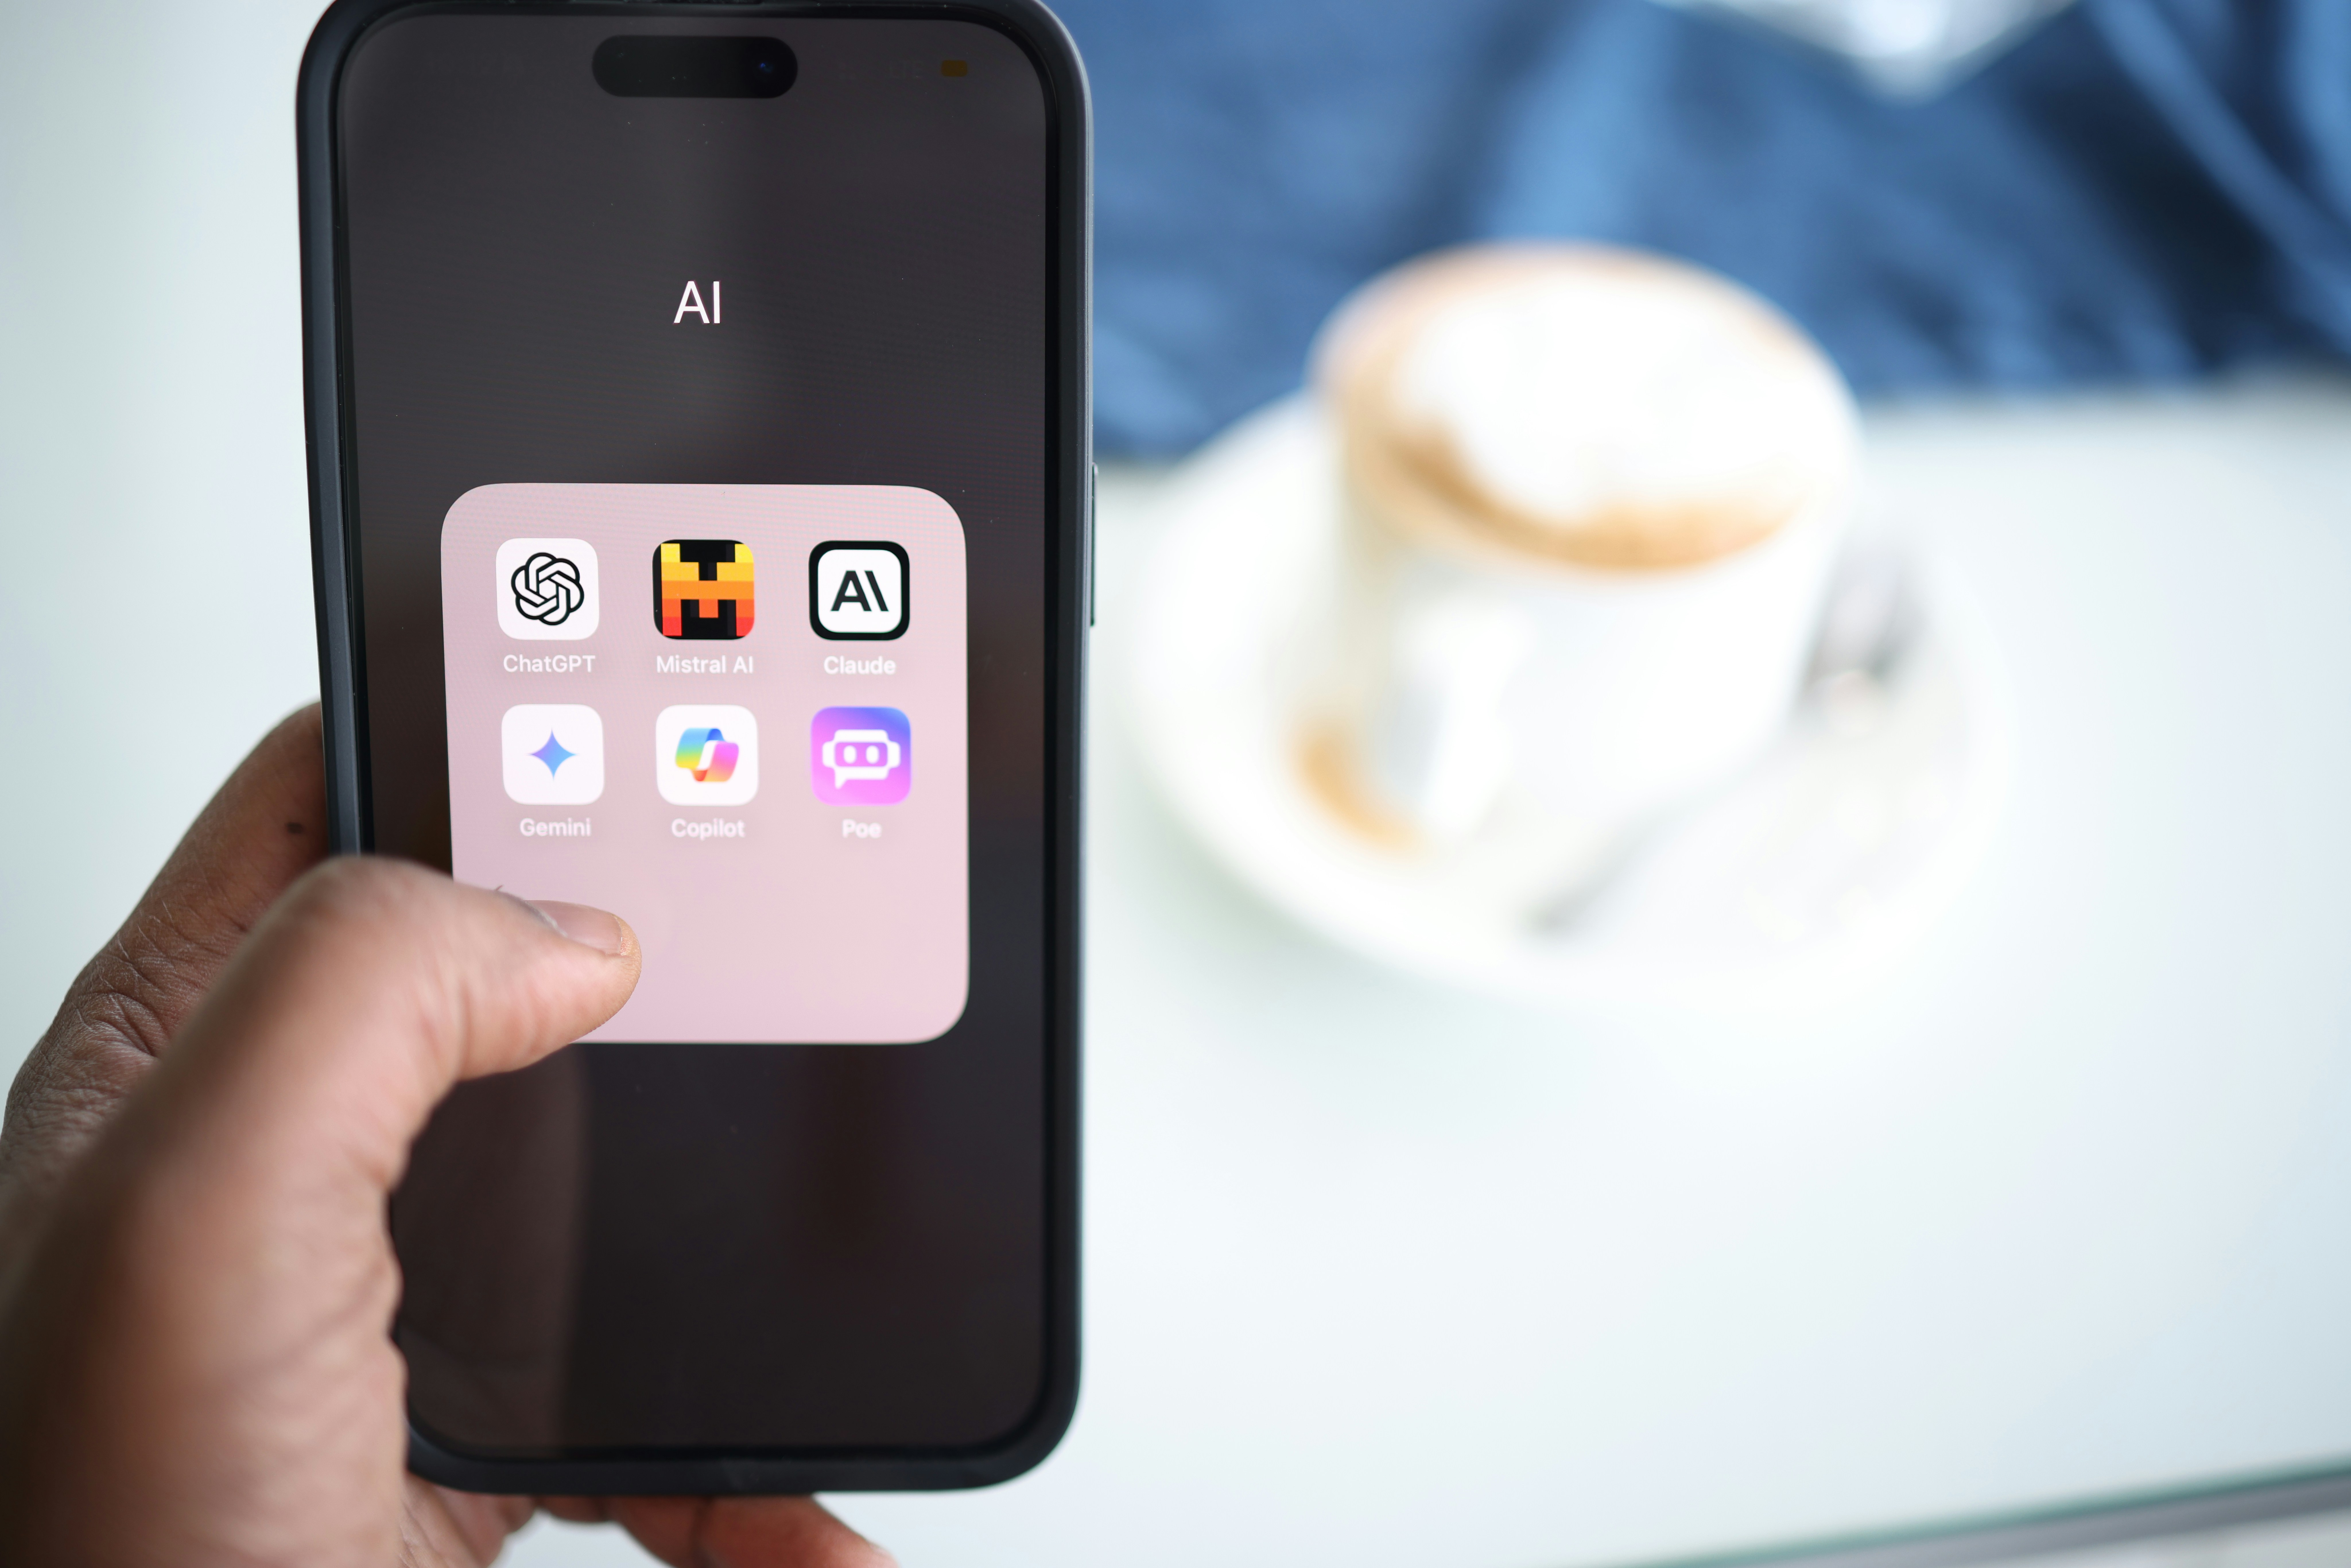
\includegraphics[width=0.6\textwidth]{static/ai-phone.jpg}\\
    \Large KI ist kein Zukunftsthema – sie ist bereits da.
\end{center}
\end{frame}

\begin{frame}{KI im Schulalltag}
      
\includegraphics[width=0.4\textwidth]{static/tungtung.png}
      
\includegraphics[width=0.5\textwidth]{static/ballerina.png}
  \begin{center}
  \begin{tiny}
    Kommt Ihnen eins dieser Bilder bekannt vor?
  \end{tiny}
\end{center}
\end{frame}

\begin{frame}{KI im Schulalltag}
\begin{center}
    \href{https://www.youtube.com/watch?v=fB_lCPFEBNU}{
        
\includegraphics[width=0.7\linewidth]{static/ballerina.png}
    }
    \vspace{0.3cm}
    \small (Klicken zum Abspielen)
\end{center}
\end{frame}

\begin{frame}{KI im Schulalltag}
  \begin{center}
      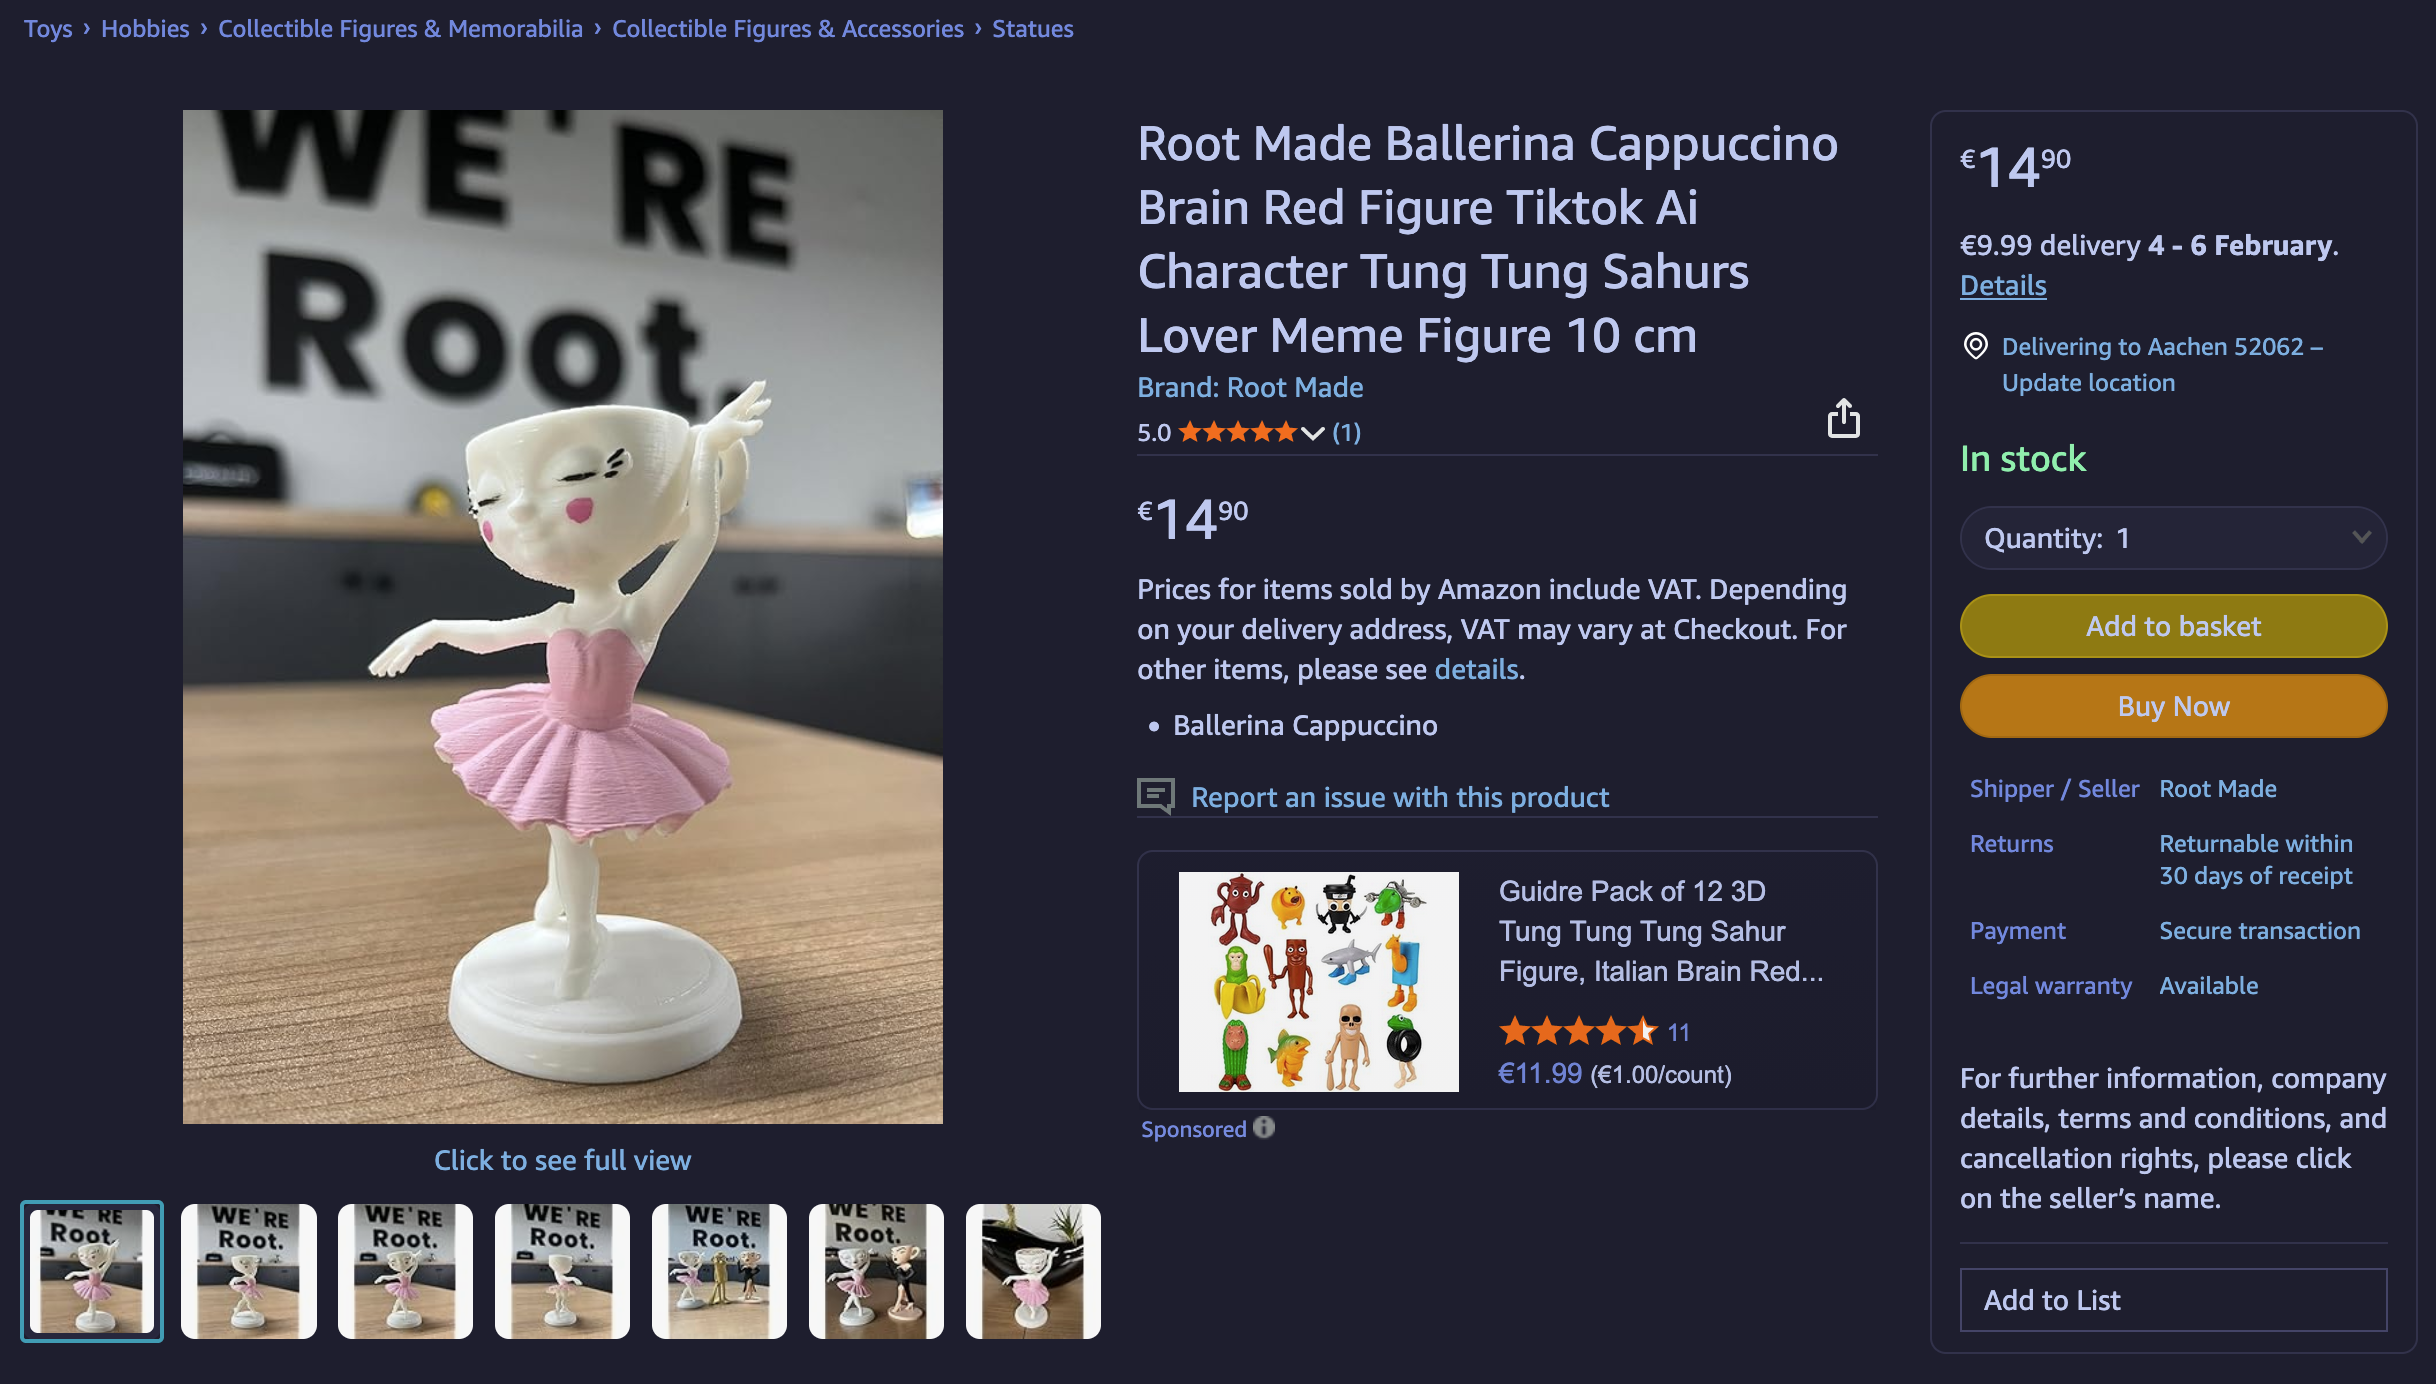
\includegraphics[width=0.9\textwidth]{static/ballerina-amazon.png}
  \begin{tiny}
  \end{tiny}
\end{center}
\end{frame}

\begin{frame}{}
\begin{center}
    \Large Frage\\
    \vspace{0.3cm}
    Wie viele Ihrer SuS haben ein Smartphone?
\end{center}
\end{frame}

\begin{frame}{KI im Schulalltag}
\begin{itemize}
    \item 65\% der 6-18-Jährigen besitzen ein Smartphone
    \item 6-9: 42\% ein eigenes Tablet, 17\% ein Smartphone
    \item 10-12: bereits 76\%!
\end{itemize}
\vspace{0.5cm}
\begin{center}
\footnotesize \autocite{ev_ab_2024}
\end{center}
\end{frame}

\begin{frame}{KI im Schulalltag}
\begin{itemize}
    \item Schüler*innen nutzen KI bereits – offen oder verdeckt
    \item Selbst junge SuS sind mit digitalen Tools vertraut
    \item \textbf{Selbst wenn nicht selbst genutzt, begegnet es ihnen}
    \item KI beeinflusst Hausaufgaben, Referate, Prüfungen
    \item Lehrkräfte stehen vor neuen Erwartungen
\end{itemize}
\end{frame}

\begin{frame}{Frage an Sie}
\begin{block}{Diskussion}
\begin{itemize}
    \item Wo begegnet Ihnen KI aktuell im Schulalltag?
\end{itemize}
\end{block}
\end{frame}


% =====================================================
% SECTION 2 – WARUM DIESES SEMINAR?
% =====================================================

\section{Warum dieses Seminar?}

\begin{frame}{}
\begin{center}
    \Large Warum dieses Seminar?\\
    Warum nicht einfach selbst ausprobieren?
\end{center}
\end{frame}

\begin{frame}{Warum nicht einfach selbst ausprobieren?}
\begin{itemize}
    \item Viele Lehrkräfte experimentieren eigenständig mit KI
    \item Ergebnisse sind oft zufällig oder wenig didaktisch fundiert
    \item Unsicherheit bleibt trotz Nutzung bestehen
    \item Massive Lücke in der Lehrkräftebildung bezüglich KI
\end{itemize}
\begin{center}
    Die meisten Studien befassen sich mit der Technik, nicht mit der Didaktik!
    \begin{tiny}
        \autocite{deriba_fairness_2025}
    \end{tiny}
\end{center}
\end{frame}

\begin{frame}{Warum nicht einfach selbst ausprobieren?}
\begin{itemize}
    \item Einzelne Tools erklären sich schnell – didaktische Einbettung nicht
    \item Gefahr von Fehlannahmen über Funktionsweise
    \item Fehlende Einordnung von Grenzen, Bias und Halluzinationen
\end{itemize}
\end{frame}

\begin{frame}{Was dieses Seminar anders macht}
\begin{itemize}
    \item Wissenschaftlich fundierte Einordnung
    \item Gemeinsame Reflexion
    \item Fokus auf nachhaltige Handlungssicherheit
\end{itemize}
\end{frame}

\begin{frame}{}
\begin{center}
    \Large Ziel ist nicht „mehr KI“
    
    \vspace{0.3cm}
    \Large sondern \textbf{bessere Entscheidungen und Umgang}, sowie \textbf{Einbau in Ihren Alltag!}.
\end{center}
\end{frame}


% =====================================================
% SECTION 3 – GRUNDLAGEN KI
% =====================================================

\section{Grundlagen: Was ist KI?}

\begin{frame}{}
\begin{center}
    \Large Grundlagen: Was ist KI?
\end{center}
\end{frame}

\begin{frame}{Was meinen wir, wenn wir von KI sprechen?}
\begin{itemize}
    \item KI ist kein Bewusstsein und kein Denken
    \item KI erkennt Muster in großen Datenmengen
    \item Entscheidungen basieren auf Wahrscheinlichkeiten
\end{itemize}
\end{frame}

\begin{frame}{KI im engeren Sinne}
\begin{itemize}
    \item Maschinelles Lernen (Machine Learning)
    \item Neuronale Netze
    \item Sprachverarbeitung (Natural Language Processing)
\end{itemize}
\end{frame}

\begin{frame}{Beispiel}
\begin{center}
    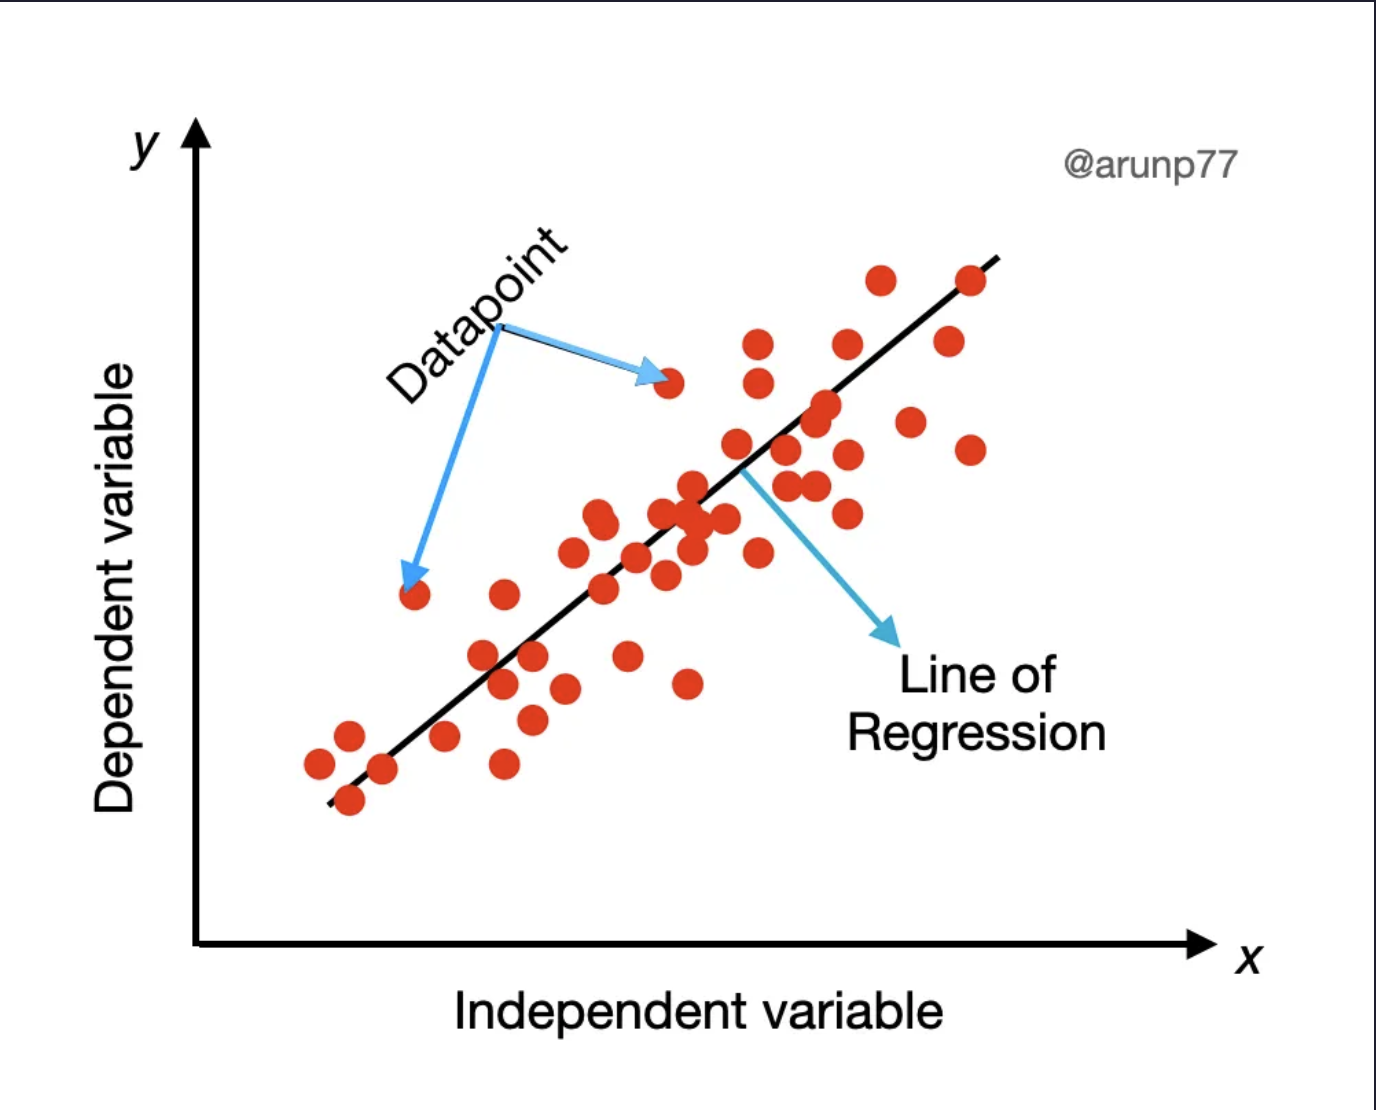
\includegraphics[width=0.6\textwidth]{static/regression.png}\\
    \vspace{0.3cm}
    \small KI versteht nicht! - sie \textbf{berechnet Wahrscheinlichkeiten}.\\
    \autocite{pandey_phd_regression_2024}
\end{center}
\end{frame}

\begin{frame}{}
\begin{center}
    \Large Was sind LLMs?
\end{center}
\end{frame}

\begin{frame}{Was sind LLMs?}
\begin{itemize}
    \item Sprachmodelle wie ChatGPT, Gemini oder Claude
    \item Trainiert auf sehr großen Textmengen
    \item Ziel: Wahrscheinlich nächstes Wort vorhersagen
\end{itemize}
\end{frame}

\begin{frame}{Wie entstehen LLMs? (vereinfacht)}
\begin{itemize}
    \item Training auf Milliarden von Textbeispielen
    \item Lernen von Sprachmustern, nicht von Wahrheit
    \item Feinjustierung durch menschliches Feedback
\end{itemize}
\end{frame}

\begin{frame}{Grenzen von LLMs}
\begin{itemize}
    \item Halluzinationen (plausibel klingende Fehler)
    \item Verzerrungen (Bias) aus Trainingsdaten
    \item Keine Quellenprüfung oder Faktenverständnis
\end{itemize}
\end{frame}

\begin{frame}{Beispiel}
\begin{center}
    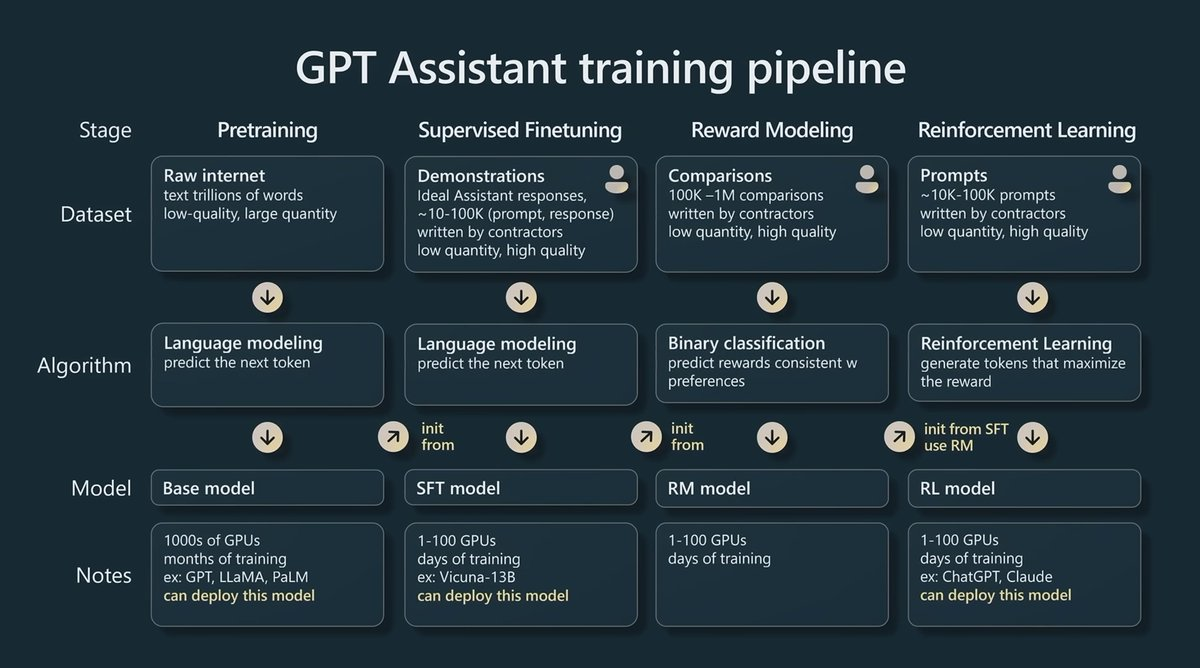
\includegraphics[width=0.8\textwidth]{static/gpt-training.jpeg}\\
    \vspace{0.3cm}
    \autocite{hasan_simple_2024}
\end{center}
\end{frame}

\begin{frame}{Beispiel}
\begin{center}
    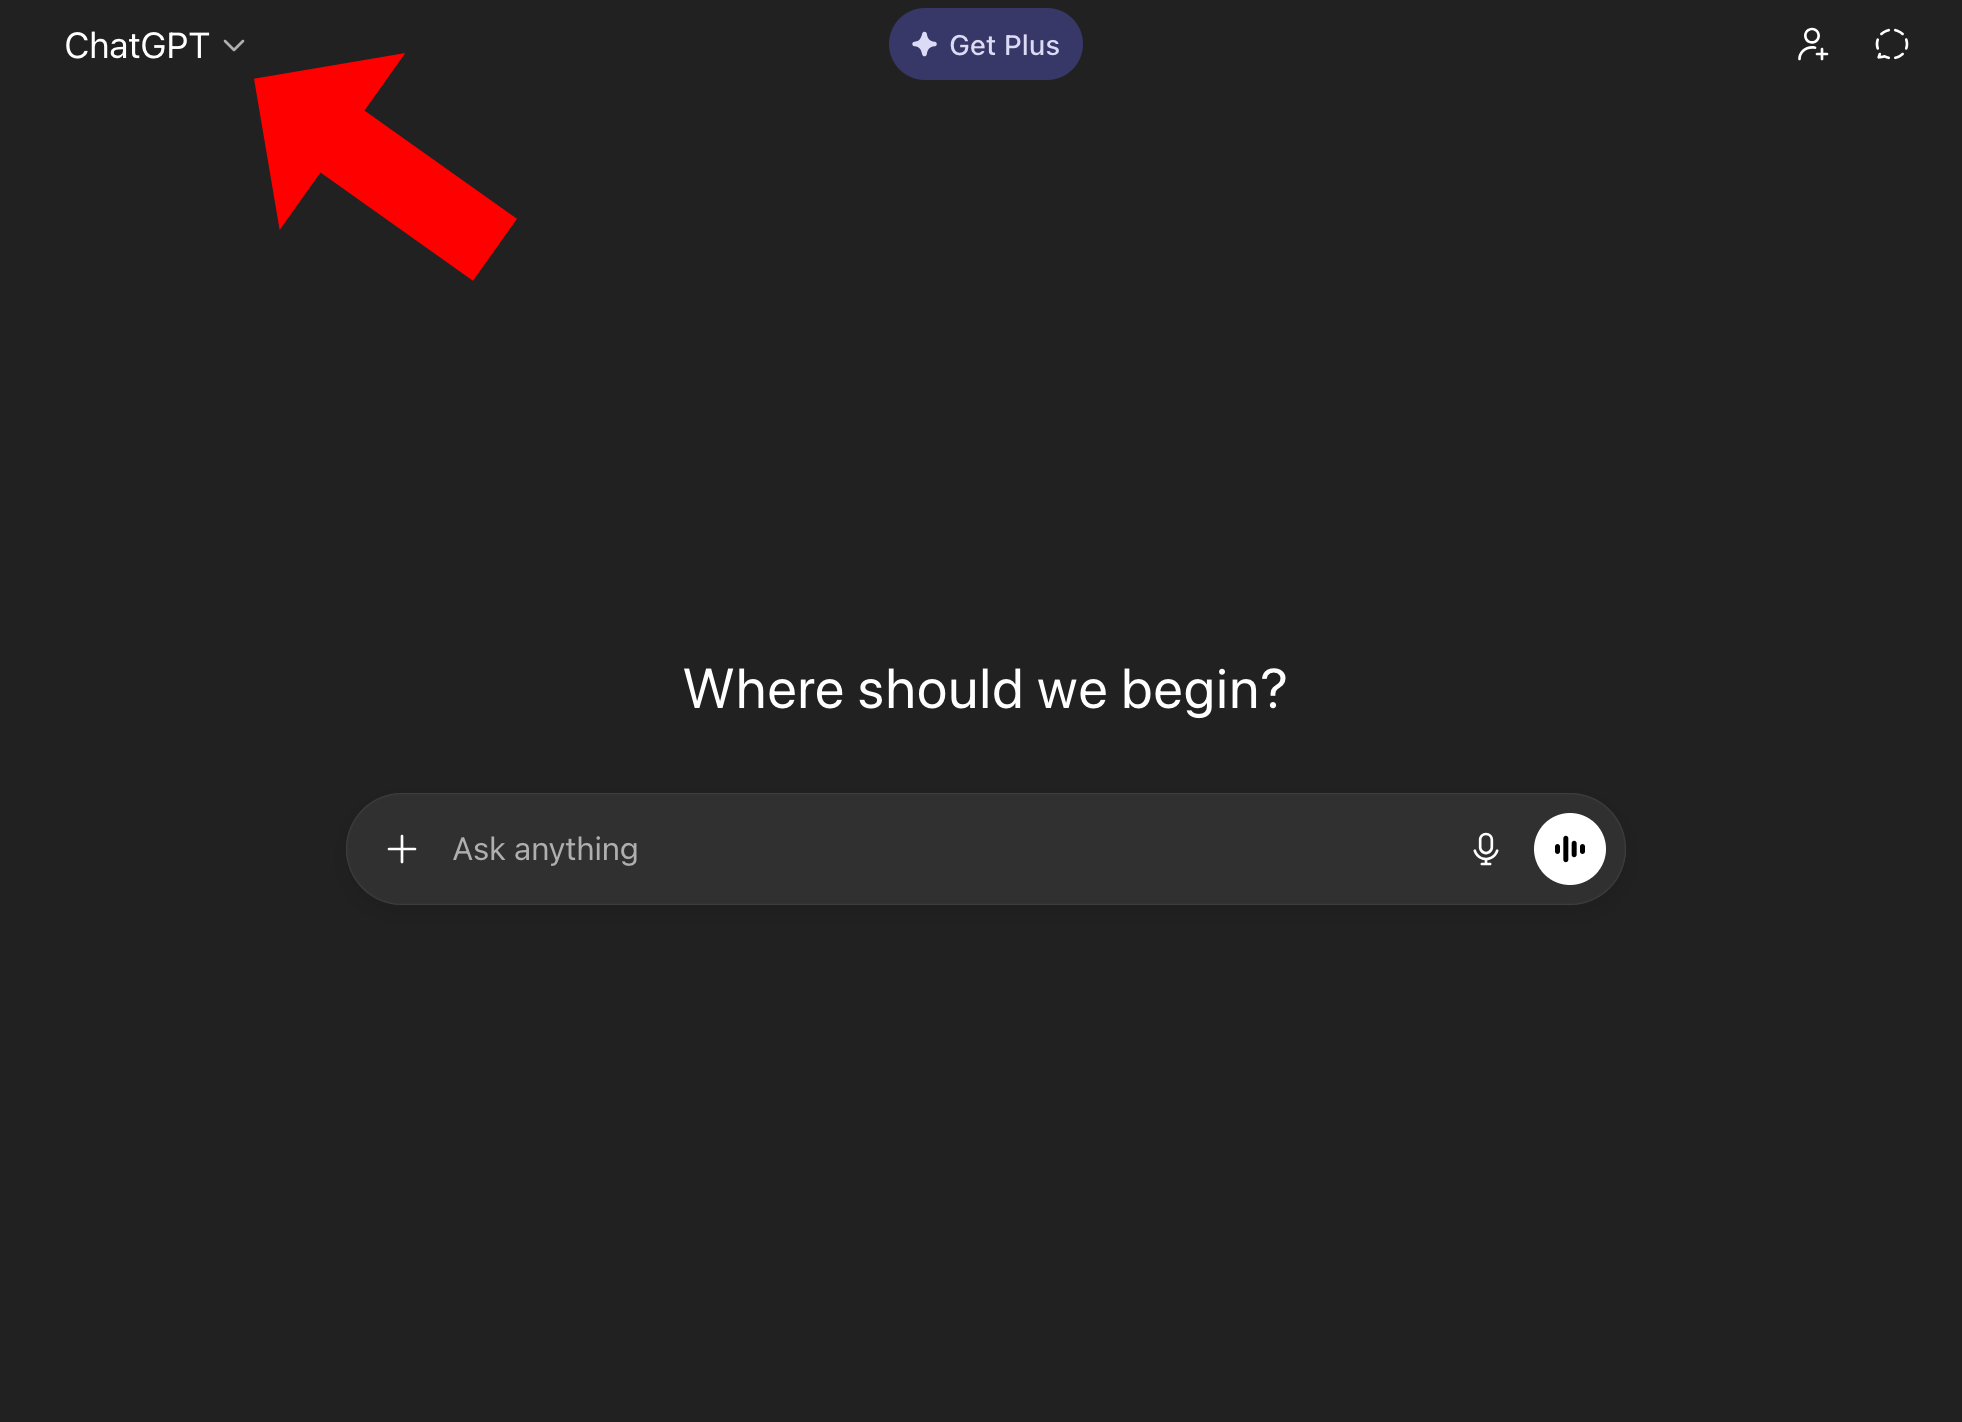
\includegraphics[width=0.75\textwidth]{static/chatgpt.png}\\
    \autocite{ai_chatgpt_nodate}
\end{center}
\end{frame}

\begin{frame}{Beispiel}
\begin{center}
    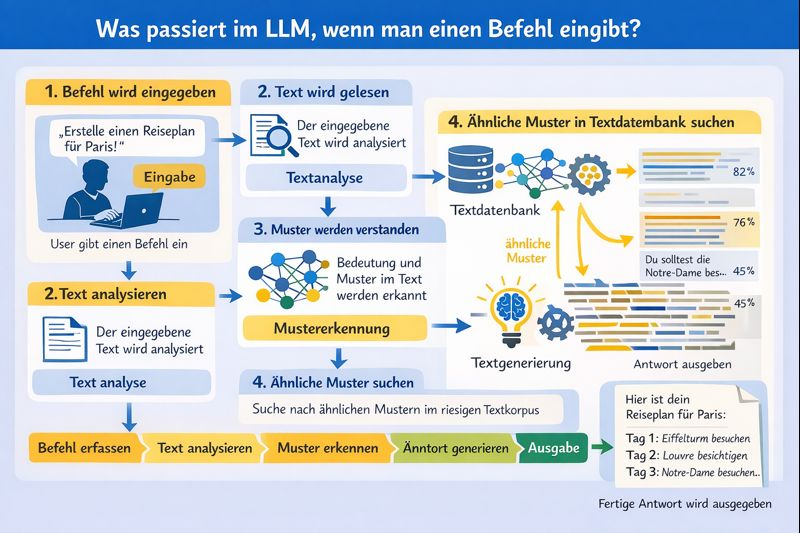
\includegraphics[width=0.9\textwidth]{static/infografik-llm.jpg}\\
\end{center}
\end{frame}

% =====================================================
% SECTION 4 – POTENZIALE
% =====================================================

\section{Potenziale}

\begin{frame}{}
\begin{center}
    \Large Was für Potenziale hat das Ganze?
\end{center}
\end{frame}

\begin{frame}{Individualisierung des Lernens}
\begin{itemize}
    \item Unterschiedliche Lernniveaus besser abbilden:
    \item Tempo, Sprache und Schwierigkeitsgrad anpassen
\end{itemize}
\end{frame}

\begin{frame}{Entlastung im Schulalltag}
\begin{itemize}
    \item Unterstützung bei Vorbereitung und Materialerstellung
    \item Zeitgewinn für pädagogische Kernaufgaben
    \item Kein Ersatz – sondern Assistenz
\end{itemize}
\end{frame}

\begin{frame}{Entlastung im Schulalltag}
\begin{itemize}
    \item Unterstützung im Unterricht:
    \item Studien zeigen, dass je nach Anwendung ein Lernerfolg durch KI-Tools erzeugt werden kann!
    \item Inklusion, vor allem für SuS mit Behinderungen!
\end{itemize}
\begin{center}
    Mehr dazu im Folgeseminar!
    \begin{tiny}
        \autocites{orhani_risks_2025}{kumar_ai_2025}
    \end{tiny}
\end{center}
\end{frame}

\begin{frame}{Frage an Sie}
\begin{block}{Reflexion}
\begin{itemize}
    \item Wo würden Sie sich im Alltag Entlastung wünschen?
\end{itemize}
\end{block}
\end{frame}

% =====================================================
% SECTION 5 – HERAUSFORDERUNGEN & STUDIEN
% =====================================================

\section{Herausforderungen \& Studien}

\begin{frame}{}
\begin{center}
    \Large Herausforderungen
\end{center}
\end{frame}

\begin{frame}{Können wir KI-Texte erkennen?}
\begin{itemize}
    \item Studien zeigen: Erkennung ist sehr schwierig
    \item Auch erfahrene Lehrkräfte liegen oft falsch
    \item Vertrauen in „Bauchgefühl“ problematisch
\end{itemize}
\end{frame}

\begin{frame}{Können wir KI-Texte erkennen?}
\begin{itemize}
    \item 289 Lehrer*innen bewerteten Texte
    \item 200 davon erfahrene Lehrkräfte
    \item Insgesamt nur 37,8\% der KI-generierten Texte korrekt erkannt
    \item Von 89 M.Ed. Studenten wurden 45.1\% der KI-Texte erkannt!
\end{itemize}
\begin{center}
\begin{tiny}
    \autocite[4f.]{fleckenstein_teachers_2024}
\end{tiny}
\end{center}
\end{frame}

\begin{frame}{Zentrale Erkenntnisse aus Studien}
\begin{itemize}
    \item KI-Texte wirken sprachlich sehr „menschlich“
    \item Detektion wird durch gezieltes Prompting erschwert
    \item Overconfidence-Effekt bei Lehrkräften
\end{itemize}
\end{frame}

\begin{frame}{Zentrale Erkenntnisse aus Studien}
 \Large Einerseits ist die Erkennung durch gezieltes Prompting erschwert,
 \vspace{0.3cm}
 \Large andererseits hilft gezieltes Prompting also auch bei der Erstellung besserer Texte.
\end{frame}

\begin{frame}{Grenzen von Erkennungstools}
\begin{itemize}
    \item Technische Detektoren sind nicht zuverlässig
    \item Hohe Gefahr von Fehlalarmen ohne gezielte Nutzung
\end{itemize}
\end{frame}

% % =====================================================
% % SECTION 6 – KONSEQUENZEN FÜR UNTERRICHT & PRÜFUNGEN
% % =====================================================
%
% \section{Konsequenzen}
%
% \begin{frame}{Was bedeutet das für uns?}
% \begin{itemize}
%     \item Fokus auf Lernprozesse statt nur Produkte
%     \item Transparente Regeln zur KI-Nutzung
%     \item Anpassung von Aufgabenformaten
% \end{itemize}
% \end{frame}
%
% \begin{frame}{Vom Schreiben zum Reflektieren}
% \begin{itemize}
%     \item KI als Diskussions- und Reflexionspartner
%     \item Analyse statt reine Textproduktion
%     \item Förderung von KI-Kompetenz
% \end{itemize}
% \end{frame}


% =====================================================
% SECTION 6 – PROMPTING
% =====================================================

\section{Prompting}
\begin{frame}{}
\begin{center}
    \Large Prompting – Der Schlüssel zu guten Ergebnissen
\end{center}
\end{frame}

\begin{frame}{Warum Prompting so wichtig ist}
\begin{itemize}
    \item KI reagiert stark auf Formulierungen
    \item Kleine Änderungen → große Ergebnisunterschiede
    \item Schlechte Prompts führen zu schlechten Ergebnissen
\end{itemize}
\end{frame}

\begin{frame}{Was ist ein Prompt?}
\begin{itemize}
    \item Eine strukturierte Arbeitsanweisung an die KI
    \item Kombination aus Rolle, Ziel und Kontext
    \item Vergleichbar mit einem sehr präzisen Befehl!
\end{itemize}
\end{frame}

\begin{frame}{Elemente eines guten Prompts}
\begin{itemize}
    \item \textbf{Rolle:} „Du bist Lehrkraft für …“
    \item \textbf{Ziel:} „Erstelle eine Unterrichtsreihe zu …“
    \item \textbf{Kontext:} Lerngruppe, Niveau, Zeitrahmen
    \item \textbf{Einschränkungen:} Lehrplan, Methoden, Sozialform
\end{itemize}
\end{frame}

\begin{frame}{Elemente eines guten Prompts}
    \textbf{Einschränkungen umgehen:} Kontext geben!!\\
    \vspace{0.3cm}
    \begin{itemize}
        \item \enquote{Berücksichtige, dass die SuS nur 30 Minuten Zeit haben.}
        \item \enquote{Die Aufgaben sollen für eine 7. Klasse geeignet sein.}
        \item \enquote{Nutze nur Quellen, die ich dir gleich gebe.}
        \item \enquote{Erstelle differenzierte Aufgaben auf Basis von... Dokument!}
    \end{itemize}
\end{frame}

% =====================================================
% SECTION 7 – PRAXISPHASE
% =====================================================

\section{Praxisphase}

\begin{frame}{}
\begin{center}
    \Large Jetzt sind Sie dran!\\
    \vspace{0.3cm}
    \normalsize Praxisphase
\end{center}
\end{frame}

\begin{frame}{Tool 1: Google NotebookLM}
\begin{itemize}
    \item Arbeiten mit eigenen Quellen
    \item Lehrpläne, Texte, PDFs einbinden
    \item KI antwortet nur auf Basis dieser Inhalte
\end{itemize}
\end{frame}

\begin{frame}{}
\begin{center}
    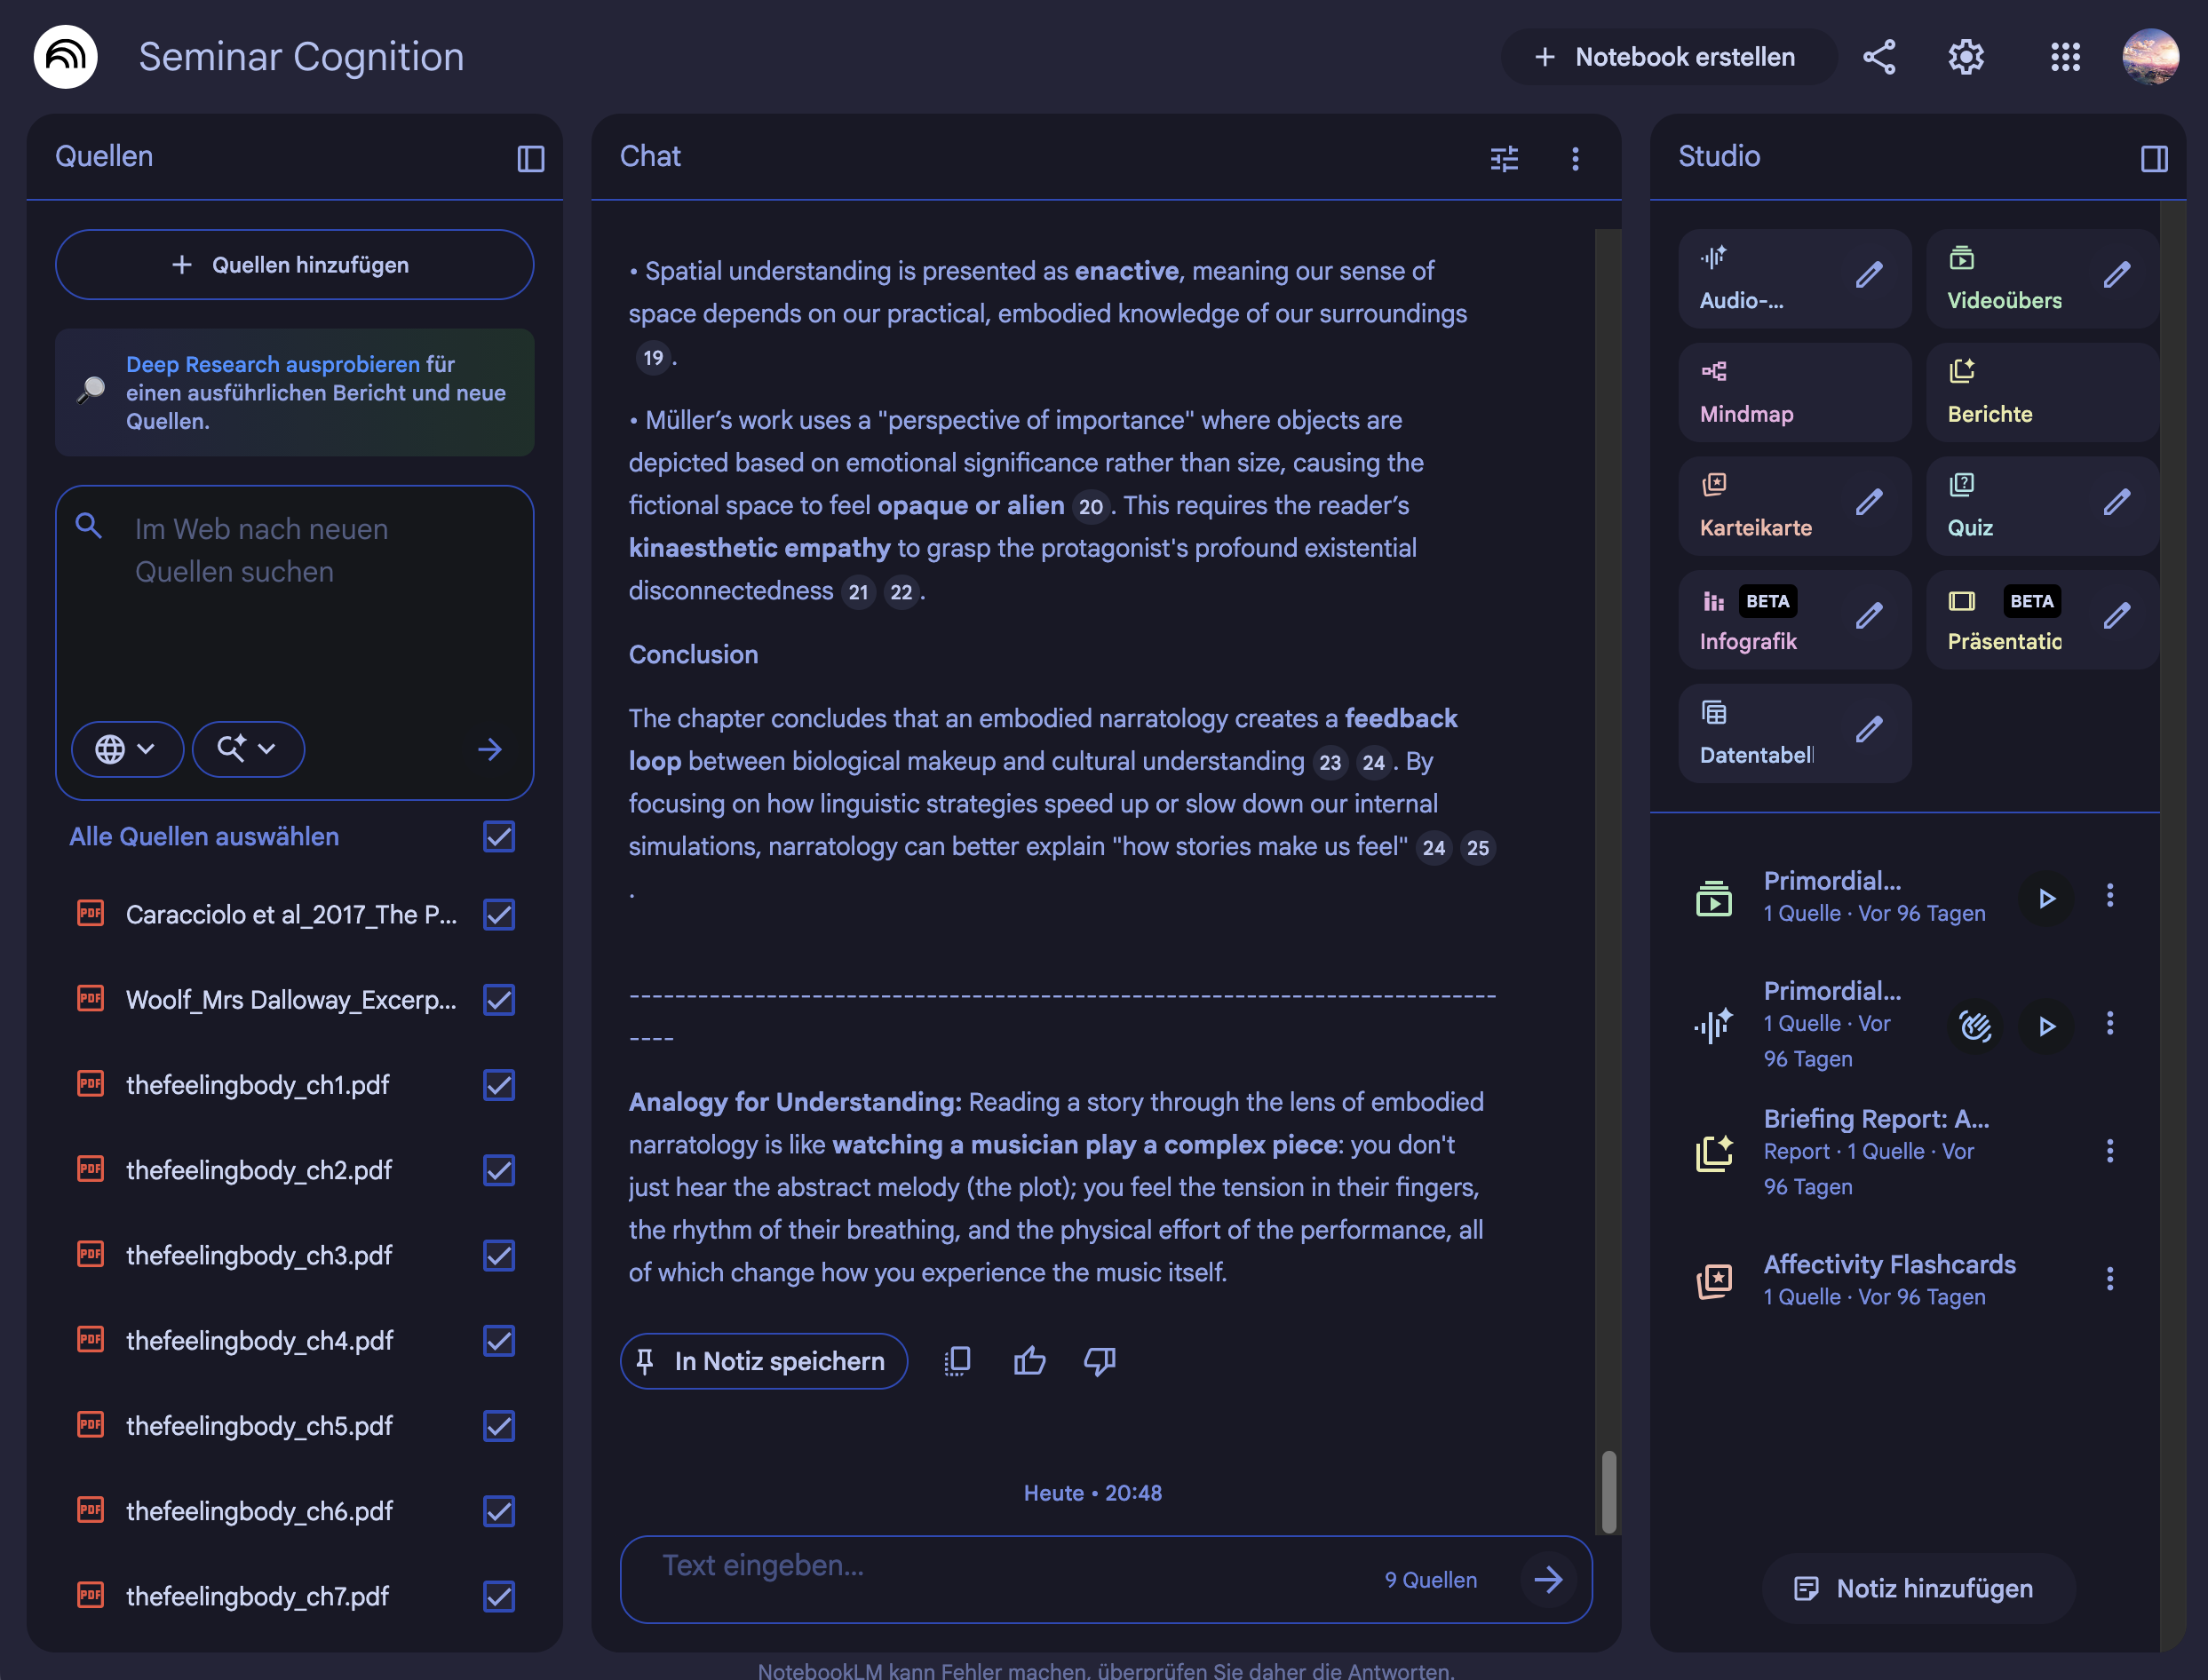
\includegraphics[width=0.7\textwidth]{static/notebooklm.png}\\
    \autocite{google_google_nodate}
\end{center}
\end{frame}

\begin{frame}{Tool 2: ChatGPT}
\begin{itemize}
    \item Ausarbeitung von Unterrichtsreihen
    \item Differenzierung und Aufgabenvarianten
    \item Reflexions- und Bewertungsfragen
\end{itemize}
\end{frame}

\begin{frame}{Recap: Prompting}
\begin{itemize}
    \item Rolle definieren (z.\,B. „Du bist Fachlehrer für …“)
    \item Ziel klar benennen
    \item Kontext, Lerngruppe und Rahmenbedingungen angeben
\end{itemize}
\end{frame}

\begin{frame}{Ihre Aufgabe (ca. 60 Minuten)}
\begin{block}{Arbeitsphase}
\begin{itemize}
    \item Entwickeln Sie eine kurze Unterrichtsreihe
    \item Nutzen Sie NotebookLM für Quellen
    \item Nutzen Sie ChatGPT für die Ausarbeitung
    \item Ergebnis: Grober Plan + 1 Beispielaufgabe
\end{itemize}
\end{block}
\end{frame}

\begin{frame}{Ihre Aufgabe (ca. 60 Minuten)}
\begin{block}{Arbeitsphase}
\begin{itemize}
    \item Laden Sie den KLP für Ihr Fach in NotebookLM hoch
    \item Entwickeln Sie für Ihr gewünschtes Thema einen passenden Prompt
    \item Denken Sie an Rolle, Ziel, Kontext und Einschränkungen
    \item Kopieren Sie das Ergebnis, und nutzen ChatGPT für die Ausarbeitung/-formulierung
    \item Wenn Plan steht: Erstellen Sie eine Beispielaufgabe
\end{itemize}
\end{block}
\end{frame}

% =====================================================
% SECTION 8 – ABSCHLUSS & AUSBLICK
% =====================================================

\section{Abschluss}

\begin{frame}{}
\begin{center}
    \Large Was Sie (hoffentlich) heute mitnehmen
\end{center}
\end{frame}

\begin{frame}{Was Sie heute mitnehmen}
\begin{itemize}
    \item Realistische Einschätzung von KI
    \item Mehr Handlungssicherheit
    \item Konkrete Ideen für den Unterricht
\end{itemize}
\end{frame}

\begin{frame}{Was Sie heute mitnehmen}
\begin{center}
    \Large Decoding\\
    \normalsize nicht nur codieren, sondern die Ergebnisse kritisch dekonstruieren und bewerten!
    \begin{tiny}
        \autocite{rahimi_ai_2025}
    \end{tiny}
\end{center}
\end{frame}

\begin{frame}{Ausblick: Level 2}
    \Large Ausblick auf weiterführende Seminare:
\begin{itemize}
    \item Fortgeschrittenes Prompting
    \item Eigene KI-Assistenten
    \item Automatisierung \& Vertiefung
\end{itemize}
\end{frame}

\begin{frame}{}
\begin{center}
    \Huge Vielen Dank!
    
    \vspace{0.5cm}
    \Large Ich freue mich auf den Austausch.
\end{center}
\end{frame}

\begin{frame}[allowframebreaks]{Literatur \& Quellen}
\printbibliography
\end{frame}

\end{document}
